% !TEX root = ../MA119-Question-Bank.tex






%%%%%%%%%List of coprime numbers < #1
% \pgfmathsetmacro{\randbound}{int(5)}



\pgfmathsetmacro{\rootSA}{int(random(2,10))}
\pgfmathsetmacro{\SideA}{int((\rootSA)^2)}
\pgfmathsetmacro{\SA}{int(5*\SideA)}
\pgfmathsetmacro{\ans}{int((\rootSA)^3)}






A cube paper box \textbf{with an open top} uses $\SA$ square centimeters paper. Find the volume of the cube. 


\begin{solution}
\begin{multicols}{2}
Suppose the length of a side of the cube is $x$ centimeters. Then the area of each side is $x^2$ square centimeters. A cube has six sides. Since the box has no top, the total side area of the box is $5x^2$ centimeters which gives the following equation
\[5x^2=\SA.\] 

\columnbreak
	\begin{center}
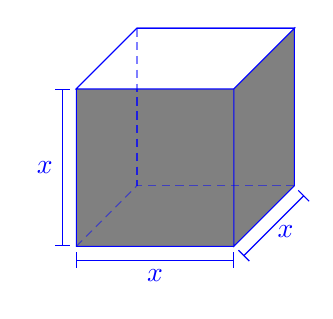
\begin{tikzpicture}[every edge quotes/.append style={auto, text=blue}]
  \pgfmathsetmacro{\cubex}{2}
  \pgfmathsetmacro{\cubey}{2}
  \pgfmathsetmacro{\cubez}{2}
  \draw [draw=blue, every edge/.append style={draw=blue, densely dashed, opacity=.5}, fill=gray]
    (0,0,0) coordinate (o) -- ++(-\cubex,0,0) coordinate (a) -- ++(0,-\cubey,0) coordinate (b) edge coordinate [pos=1] (g) ++(0,0,-\cubez)  -- ++(\cubex,0,0) coordinate (c) -- cycle
    (o) -- ++(0,0,-\cubez) coordinate (d) -- ++(0,-\cubey,0) coordinate (e) edge (g) -- (c) -- cycle
    (o) -- (a) -- ++(0,0,-\cubez) coordinate (f) edge (g) -- (d) -- cycle;
  \path [every edge/.append style={draw=blue, |-|}]
    (b) +(0,-5pt) coordinate (b1) edge[below] node[blue]{$x$} (b1 -| c)
    (b) +(-5pt,0) coordinate (b2) edge[left] node[blue]{$x$} (b2 |- a)
    (c) +(3.5pt,-3.5pt) coordinate (c2) edge[right, pos=0.4] node[blue]{$x$} ([xshift=3.5pt,yshift=-3.5pt]e)
    ;
  \draw [draw=blue, every edge/.append style={draw=blue, densely dashed, opacity=.5}, fill=white]
    (o) -- (a) -- ++(0,0,-\cubez) coordinate (f) edge (g) -- (d) -- cycle;
\end{tikzpicture}
	\end{center}	
\end{multicols}

Solve the equation to find $x$.
\[
\begin{split}
  5x^2&=\SA\\
x^2&=\SideA\\
x^2-\SideA=0\\
(x-\rootSA)(x+\rootSA)&=0\\
\end{split}
\]
Then 
\begin{alignat*}{3}
    x&=\rootSA && \ctc{or} & x&=-\rootSA
\end{alignat*}
So the length of each side is $\rootSA$ centimeters and the volume is $\rootSA^3=\ans$ cubic centimeters.
\end{solution}